% +--------------------------------------------------------------------+
% | LaTeX Template                                                     |
% | for K-State Electronic Theses, Dissertations, and Reports          |
% |                                                                    |
% | Comments and guidelines for using the template are shown           |
% | within boxes like this one.                                        |
% |                                                                    |
% | Revised 6/30/06                                                    |
% | 9/14/06: Removed typos                                             |
% +--------------------------------------------------------------------+

% +--------------------------------------------------------------------+
% | Your paper should contain the following sections, except where     |
% | indicated as optional, in the order shown.  Also, all headings     |
% | shown with an asterisk (*) must be centered and in uppercase       |
% | letters:                                                           |
% |                                                                    |
% | Abstract Title Page (doctoral dissertations only)                  |
% | ABSTRACT* (doctoral dissertations only)                            |
% | Title Page                                                         |
% | Copyright Page (Optional - only needed if copyrighting)            |
% | ABSTRACT *                                                         |
% | TABLE OF CONTENTS *                                                |
% | LIST OF FIGURES *                                                  |
% | LIST OF TABLES*                                                    |
% | ACKNOWLEDGMENTS* (Optional)                                        |
% | DEDICATION * (Optional)                                            |
% | PREFACE * (Optional)                                               |
% | Individual Chapters                                                |
% | References and/or bibliography                                     |
% | Appendices (as needed)                                             |
% +--------------------------------------------------------------------+

% +--------------------------------------------------------------------+
% | The LaTex keyword \documentclass selects a particular class to     |
% | associate with the document.  The current documentclass            |
% | {class_diss} generates a Table of Contents that has leading dots   |
% | only on chapter subheadings.  If you prefer a Table of Contents    |
% | that has leading dots for all entries, replace {class_diss}        |
% | with {Mydiss} in the command below.                                |
% |                                                                    |
% +--------------------------------------------------------------------+

\documentclass[final, 12pt,oneside]{class_diss}

% +--------------------------------------------------------------------+
% | The following command sets the bibliography style to American
% | Institute of Physics (AIP).  Other styles are available in the
% | styles directory.  To use a different style, replace "aip" with
% | the filename of the style you want to use.
% +--------------------------------------------------------------------+

\bibliographystyle{styles/plain}

\usepackage[utf8]{inputenc}
\usepackage[T1]{fontenc}
\usepackage[spanish]{babel}
% +--------------------------------------------------------------------+
% | Now, we add in all external packages that we will use throughout   |
% | the document.  You can add other packages as needed.
% +--------------------------------------------------------------------+

%\usepackage{     caption2} % Customize captions a bit more
\usepackage{      amsmath} % American Mathematics Society standards
%\usepackage{      wrapfig} % Wraps text around a figure or table
\usepackage{     graphicx} % Extended graphics package.
%\usepackage{     fancyhdr} % Efficiently handles headers and footers
%\usepackage{       braket} % Bra-Ket notation package
%\usepackage{     mathrsfs} % Specialized Math fonts (Hamiltonian, etc.)
%\usepackage{boxedminipage} % Boxed text can be produced
%\usepackage{     setspace} % Controls line spacing via \begin{space}

\usepackage{amsxtra}
\usepackage{amssymb}
\usepackage{amsthm}
\usepackage{latexsym}

% +--------------------------------------------------------------------+
% | The color package allows one to select colors for hyperlinking     |
% | (see below).                                                       |
% +--------------------------------------------------------------------+

\usepackage[usenames]{color}

% +--------------------------------------------------------------------+
% | Colors defined for use with this template.                         |
% +--------------------------------------------------------------------+

\definecolor{  Pink}{rgb}{1.0, 0.5, 0.5}
\definecolor{Maroon}{rgb}{0.8, 0.0, 0.0}

% +--------------------------------------------------------------------+
% | In the commands below, we use the 'natbib' package, and specify    |
% | the 'sort&compress' option, which condenses                        |
% | citations from (1,2,3,5,9,10,11) to (1-3,5,9-11).  The 'bibpunct'  |
% | option selects various parameters for how the citation will be     |
% | displayed.  In this case, only the comma (separation between       |
% | citations) and the 's' (superscript) arguments are chosen.  The    |
% | other curly braces deal with how to 'wrap' the citation (using     |
% | parentheses, brackets, etc.) and are not needed for the chosen     |
% | style.                                                             |
% +--------------------------------------------------------------------+

\usepackage[sort&compress]{natbib}
\bibpunct{}{}{,}{s}{}{}
\usepackage{hypernat}

% +--------------------------------------------------------------------+
% | Lastly, the hyperref package allows one to hyperlink cross-        |
% | references and figures in a LaTeX document.                        |
% +--------------------------------------------------------------------+

\usepackage[pdftex, plainpages=false, pdfpagelabels]{hyperref}

\hypersetup{
    linktocpage=true,
    colorlinks=true,
    %bookmarks=true,
    citecolor=green,
    urlcolor=blue,
    linkcolor=magenta,
    citebordercolor={1 0 0},
    urlbordercolor={1 0 0},
    linkbordercolor={.7 .8 .8},
    breaklinks=true,
    %pdfpagelabels=true,
    }

% +--------------------------------------------------------------------+
% | Page margins are set on 1 inch on all sides.                       |
% +--------------------------------------------------------------------+

\topmargin      = -0.56in
\textheight     =  8.60in
\textwidth      =  6.46in
\oddsidemargin  =  0.02in

% +--------------------------------------------------------------------+
% | The document finally begins here.                                  |
% +--------------------------------------------------------------------+

\begin{document}


  \setcounter{page}{-1}


% +--------------------------------------------------------------------+
% | Title Page -- Required for both Doctoral and Masters Students
% +--------------------------------------------------------------------+

% +--------------------------------------------------------------------+
% | Title Page
% +--------------------------------------------------------------------+

\newpage

% +--------------------------------------------------------------------+
% | This page should not contain a page number.  We use the
% | \thispagestyle[empty] command below to suppress page numbers
% | and other style elements.
% +--------------------------------------------------------------------+

\thispagestyle{empty}

% +--------------------------------------------------------------------+
% | The Title page begins here.
% +--------------------------------------------------------------------+

\begin{center}

   \vspace{1cm}

% +--------------------------------------------------------------------+
% | On the line below, replace "ENTER YOUR TITLE" with the title of
% | your ETDR.  Use all CAPITAL LETTERS.
% +--------------------------------------------------------------------+

   {\Large Suite de domótica libre}\\

   \vspace{1cm}

   {\large
    Sergio Calero Robles\\
    Diego Valbuena Pineda\\
    }

   \vspace{0.5cm}




   GRADO DE INGENIERIA INFORMÁTICA. FACULTAD DE INFORMÁTICA\\
   UNIVERSIDAD COMPLUTENSE DE MADRID \\


   \vspace{0.65cm}
   \rule{2in}{0.5pt}\\
   \vspace{0.85cm}

  
\includegraphics[height=2.5in]{figures/escudo.jpg}


%+-- Escribe el nombre de tu asignatura de fin de master (Ingeniería de computadores,....)
   \vspace{0.5cm}
    Trabajo Fin grado en Ingeniería Informática

   \vspace{0.5cm}





% +--------------------------------------------------------------------+
%  Fecha
% +--------------------------------------------------------------------+

  04/10/2018\\
   \vspace{1cm}

\end{center}

{\raggedleft
Director:\\
   \vspace{ 1cm}
Jorge Gomez Sanz\\

}
% +--------------------------------------------------------------------+
% | Use the section below if you have co-major professors.
% +--------------------------------------------------------------------+

%\begin{flushleft}
%   \hspace{10cm}Approved by:\\
%   \vspace{ 1cm}
%   \hspace{10cm}Co-Major Professor\\
%   \hspace{10cm}Enter Your Co-Major Professor's Name\\
%   \vspace{.5cm}
%   \hspace{10cm}Co-Major Professor\\
%   \hspace{10cm}Enter Your Co-Major Professor's Name\\
%\end{flushleft}

% +--------------------------------------------------------------------+
%  Pagina en Blanco con aviso de impresión
% +--------------------------------------------------------------------+

\clearpage

\thispagestyle{empty}

\begin{center}

{ Documento maquetado con \LaTeX{} }

\vfill
{Este documento está preparado para ser impreso a doble cara.}

\end{center}

   \pdfbookmark[0]{Portada}{PDFPortadaPage}

% +--------------------------------------------------------------------+
% | Autorizacion Page -- Required for both Doctoral and Masters Students
% +--------------------------------------------------------------------+

% +--------------------------------------------------------------------+
% | Copyright Page
% +--------------------------------------------------------------------+

\newpage

\thispagestyle{empty}

\begin{center}

{\bf \Huge Autorización de difusión}

\vspace{1cm}

% +--------------------------------------------------------------------+
% | On the line below, replace "Enter Your Name" with your name
% | Use the same form of your name as it appears on your title page.
% | Use mixed case, for example, Lori Goetsch.
% +--------------------------------------------------------------------+

   \large Autores\\
   \vspace{0.5cm}
    Sergio Calero Robles\\
    Diego Valbuena Pineda\\
   \vspace{0.5cm}

% +--------------------------------------------------------------------+
% | On the line below, replace Fecha
% |
% +--------------------------------------------------------------------+

   Fecha\\
   01/09/2019

   \vspace{0.5cm}
   \end{center}
   
Los abajo firmantes, matriculados en el grado en Informática de la Facultad de Informática, autorizan a la Universidad Complutense de Madrid (UCM) a difundir y utilizar con fines académicos, no comerciales y mencionando expresamente a sus autores el presente Trabajo Fin de Grado: “TÍTULO”, realizado durante el curso académico 2018-2019 bajo la dirección de J. Gomez-Sanz [y con la colaboración externa de dirección de YYYY] en el Departamento de Ingeniería de Software e Inteligencia Artifical, y a la Biblioteca de la UCM a depositarlo en el Archivo Institucional E-Prints Complutense con el objeto de incrementar la difusión, uso e impacto del trabajo en Internet y garantizar su preservación y acceso a largo plazo.


   \pdfbookmark[0]{Autorización}{PDFAutorizacionPage}


   % +--------------------------------------------------------------------+
% | Dedication Page (Optional)
% +--------------------------------------------------------------------+

\newpage

\thispagestyle{empty}
\begin{center}

{\bf \Huge Prólogo}
\end{center}
\vspace{1cm}

%\pdfbookmark[0]{Prologue}{PDF_Prologue}

% +--------------------------------------------------------------------+
% | Enter the text for your dedication in the space below this box.
% +----------------
La domótica, comúnmente asociada al confort en la vivienda. Persianas que suben y bajan a golpe de interruptor, luces que se encienden al pasar, equipos de climatización controlados mediante termostatos y una infinita lista de automatismos en dispositivos o la propia infraestructura del hogar. Esta comodidad generalmente está acompañada de restricciones técnicas y económicas para la mayoría de la gente, por ello, la domótica ha terminado como uno de esos elementos distintivos de la sociedad de elite que se lo puede permitir.

La abundante proliferación de dispositivos electrónicos en el hogar en las últimas décadas ha planteado la interconexión de los mismos en sistemas centralizados con control remoto. El confort que en el milenio pasado estaba reservado a una terminal en alguna pared de la vivienda, que permitía gestionar los costosos automatismos ahora pueden ser manejados desde un simple smartphone para hacer, por ejemplo, unas tostadas.

Y ahora todo está interconectado, si no, pregunten a cierta empresa china cuyo “grano de arroz de un budista es tan grande como una montaña”, la cual insiste en que hasta mis zapatillas tengan WiFi. Bien, es evidente e imparable la interconexión de todos los dispositivos del planeta a la obra de ingeniería más grande de la humanidad. Es por ello han nacido términos como el Internet de las cosas o el fogging.

Por supuesto hay motivaciones para esta aparente necesidad de conectividad de sensores y actuadores, se ven reflejadas en el nacimiento de la industria 4.0 y ya hay quien habla de humanidad 2.0. Recolectar ingentes volúmenes de datos para luego realizar estudios conductuales, o previsiones de mercado, son algunas de las aplicaciones más demandadas en nuestra era.La domótica, en este sentido puede beneficiarse de estos avances para proporcionar automatismos mas allá del confort, esto es, por ejemplo, para cuidar el medio ambiente y de paso, nuestro bolsillo. Un argumento aparentemente inconexo, pero este documento, aparte de cubrir los aspectos esperados en un TFG, demostrara que ciertamente hay mucho beneficio, al alcance de buena parte de la población mundial, con la automática en el hogar.

   % +--------------------------------------------------------------------+
% | Copyright Page
% +--------------------------------------------------------------------+

\newpage

\thispagestyle{empty}

\begin{center}

{\bf \Huge Resumen en castellano}

  \end{center}
\vspace{1cm}

Proceso documentado paso a paso de la implantación y puesta en marcha de un sistema modular de domótica integrada. Criterios y selección de hardware necesario, instalación y configuración del software, implementación del código fuente y compilación necesarios para dar operatividad al sistema y definición y creación de los modulos disponibles asi como sus posibles configuraciones.

\vspace{1cm}

% +--------------------------------------------------------------------+
% | On the line below, repla	ce Fecha
% |
% +--------------------------------------------------------------------+

\begin{center}

{\bf \Large Palabras clave}

   \end{center}

   \vspace{0.5cm}
   
   Lista de palabras clave
   



   
   \pdfbookmark[0]{Resumen}{PDFResumenPage}

    % +--------------------------------------------------------------------+
% | Copyright Page
% +--------------------------------------------------------------------+

\newpage

\thispagestyle{empty}

\begin{center}

{\bf \Huge Abstract}

  \end{center}
\vspace{1cm}

Document

\vspace{1cm}

% +--------------------------------------------------------------------+
% | On the line below, replace Fecha
% |
% +--------------------------------------------------------------------+

\begin{center}

{\bf \Large Keywords}

   \end{center}

   \vspace{0.5cm}
   
List of keywords
   



       \pdfbookmark[0]{Abstract}{PDFAbstractPage}
    \vfill


% +--------------------------------------------------------------------+
% | We use the following code to suppress page numbers and other
% | style issues we do not want present on a given page.               |
% +--------------------------------------------------------------------+

%\thispagestyle{empty} Looks like it's ok to remove this line
\newpage
\pagenumbering{roman}

% +--------------------------------------------------------------------+
% | On the line below, set the number to represent the page number of
% | the Table of Contents page.  For example, if the Table of Contents
% | page is the 8th page of your document, enter 8 in the brackets.  This
% | number may vary, depending on the length of your abstract.
% |
% | Numbers do not appear on the title and abstract pages, but they are
% | included in the page count.  The Table of Contents page is the
% | first page on which page numbers are displayed.
% +--------------------------------------------------------------------+

\setcounter{page}{1}

% +--------------------------------------------------------------------+
% | Here, we will generate our Table of Contents (TOC) entries.        |
% | This adds the section to the TOC and then generates the indicated  |
% | section.                                                           |
% +--------------------------------------------------------------------+

\phantomsection
\addcontentsline{toc}{chapter}{Índice}

\tableofcontents
%\listoffigures
%\listoftables

%\hfill  Are these lines necessary?
%\hfill

% +--------------------------------------------------------------------+
% | Acknowledgements Page
% |
% | If you choose not to have an Acknowledgements page, comment out
% | or delete the following 3 lines.
% +--------------------------------------------------------------------+

% +--------------------------------------------------------------------+
% | Acknowledgements Page (Optional)                                   |
% +--------------------------------------------------------------------+

\newpage
\begin{center}
{\bf \Huge Agradecimientos}
\end{center}
\vspace{1cm}
\setlength{\baselineskip}{0.8cm}

%\pdfbookmark[0]{Acknowledgements}{PDF_Acknowledgements}

% +--------------------------------------------------------------------+
% | Enter text for your acknowledgements in the space below this box.  |
% |                                                                    |
% +--------------------------------------------------------------------+

Es nuestro deseo aprovechar este espacio para agradecer al equipo docente de la Facultad de Informática, pues siempre hemos valorado positivamente el esfuerzo y dedicación que han invertido en todos los estudiantes y con ello se han ganado nuestro respeto y admiración. También estamos en deuda con nuestros más cercanos compañeros de carrera, gracias a los cuales hemos reforzado nuestras aptitudes, superado obstáculos, y encontrado motivación y nuevas energías cuando hicieron falta. Tendréis nuestro respeto y aprecio allá donde estéis. Un agradecimiento especial a nuestros familiares y nuestras parejas, que siempre han estado apoyándonos y velando por nuestros intereses, pese a nuestras diferencias, que ponen de manifiesto la evidente suerte que nos ha tocado en la vida. Y expresar también el orgullo de haber sido tutelados por el Dr. Jorge Gomez Sanz, sus ánimos y templanza han hecho que este trabajo de fin de grado haya sido un éxito personal para nosotros.

\phantomsection
\addcontentsline{toc}{chapter}{Agradecimientos}

% +--------------------------------------------------------------------+
% | Dedication Page
% |
% | If you choose not to have a Dedication page, comment out
% | or delete the following 3 lines.
% +--------------------------------------------------------------------+

% +--------------------------------------------------------------------+
% | Dedication Page (Optional)
% +--------------------------------------------------------------------+

\newpage

%\pdfbookmark[0]{Dedication}{PDF_Dedication}

% +--------------------------------------------------------------------+
% | Enter the text for your dedication in the space below this box.
% +----------------
\textit{Qué hermoso es hablarle a la máquina en su propio idioma, y que nos responda en el nuestro}

\textbf{Cid Meier's Civilization®: Beyond Earth}

\phantomsection
\addcontentsline{toc}{chapter}{Dedicatoria}

% +--------------------------------------------------------------------+
% | Preface Page
% +--------------------------------------------------------------------+

%% +--------------------------------------------------------------------+
% | Preface (Optional)
% +--------------------------------------------------------------------+

\newpage
\begin{center}
{\bf \Huge Preface}
\end{center}
\vspace{1cm}
\setlength{\baselineskip}{0.8cm}

%\pdfbookmark[0]{Preface}{PDF_Preface}

% +--------------------------------------------------------------------+
% | Enter text of your Preface in the space below this box.
% +--------------------------------------------------------------------+

This template uses a separate file for each section of your ETDR:
title page, abstract, preface, chapters, reference, etc.  This
makes it easier to organize and work with a lengthy document.  The
template is configured with page margins required by the Graduate
School and will automatically create a table of contents, lists of
tables and figures, and PDF bookmarks.

Although the template gives you a foundation for creating your
ETDR, you will need a working knowledge of LaTeX in order to
produce a final document.  You should be familiar with LaTeX
commands for formatting text, equations, tables, and other
elements you will need to include in your ETDR.

This template uses a separate file for each section of your ETDR:
title page, abstract, preface, chapters, reference, etc.  This
makes it easier to organize and work with a lengthy document.  The
template is configured with page margins required by the Graduate
School and will automatically create a table of contents, lists of
tables and figures, and PDF bookmarks.

Although the template gives you a foundation for creating your
ETDR, you will need a working knowledge of LaTeX in order to
produce a final document.  You should be familiar with LaTeX
commands for formatting text, equations, tables, and other
elements you will need to include in your ETDR.

This template uses a separate file for each section of your ETDR:
title page, abstract, preface, chapters, reference, etc.  This
makes it easier to organize and work with a lengthy document.  The
template is configured with page margins required by the Graduate
School and will automatically create a table of contents, lists of
tables and figures, and PDF bookmarks.

Although the template gives you a foundation for creating your
ETDR, you will need a working knowledge of LaTeX in order to
produce a final document.  You should be familiar with LaTeX
commands for formatting text, equations, tables, and other
elements you will need to include in your ETDR.

%\phantomsection
%\addcontentsline{toc}{chapter}{Preface}

% +--------------------------------------------------------------------+
% | We use arabic (1, 2, 3...) page numbering starting from page 1.    |
% | Note, however, that there are many pages where this is not the     |
% | desired behavior - such as the Title page, or abstract.  In these  |
% | cases, we can use \thispagestyle{empty} to suppress page numbers,  |
% | and other general style issues that we've defined globally.        |
% +--------------------------------------------------------------------+

\newpage
\pagenumbering{arabic}
\setcounter{page}{1}

% +--------------------------------------------------------------------+
% | Here is where we include individual sections of the thesis or
% | dissertation.                                                      |
% +--------------------------------------------------------------------+

% +--------------------------------------------------------------------+
% | Chapters
% +--------------------------------------------------------------------+

\cleardoublepage

\chapter{Introducción}

\section{Presentación de proyecto}
\label{ch:Capitulo1}
El presente documento recoge el proceso de creación de un prototipo como solución integral de domótica programable, gestionada mediante software para plataforma móvil y Web App. La naturaleza del proyecto posee una vertiente asequible y libre. Para poder cumplir con estos objetivos, será necesario que los materiales y dispositivos utilizados para su implementación sean sencillos de adquirir, fáciles de reemplazar, además de tener un bajo coste en precio de adquisición y de tiempo necesario para su instalación, todo ello usando como base software y hardware libre.

\section{Motivación}
\label{ch:Capitulo1.1}

En los últimos años, la domótica ha sufrido un crecimiento acelerado gracias a la interconexión de dispositivos IoT con aplicaciones móviles. Se venden kits de domótica $Plug and Play$, que requieren únicamente de la instalación de una aplicación de movil gratuita y la adquisición de los productos ofertados por los fabricantes que operen en las plataformas de dichas aplicaciones. Una gran competencia entre empresas a surgido a raíz de este planteamiento, ofreciendo una gama extensa de dispositivos y electrodomésticos que pueden combinarse, en algunos casos incluso, interoperar entre los distintos ecosistemas. Esta disputa se está desarrollando en una etapa de incertidumbre, causada por la fase experimental de productos que se ofertan a los consumidores, ya que aún no existe una necesidad real de domótica en las personas, como ocurre, por ejemplo, con los smartphones o tables. Se siguen buscando estrategias de marketing para crear dicha necesidad mediante productos que aportan confort, tomemos por ejemplo los sistemas de iluminación con múltiples configuraciones de intensidad, o traking de actividad, históricos de peso en una báscula. Independientemente de las ideas presentadas ya se están estableciendo unas pautas comunes en todos los actores del sector de la domótica. Es en estas pautas donde aparece nuestra preocupación a la hora de optar por las soluciones con más presencia del mercado (véase Xiamoi, Amazon o Google) que motivan la búsqueda de una suite de domótica que se aleje de los siguientes planteamientos.

En primer lugar, la tendencia es ofrecer dispositivos de distintos rangos de precio, que están diseñados para utilizarse cada uno en los propios ecosistemas privativos de cada marca. Implica supeditarse a las imposiciones técnicas que cada fabricante decida ofrecer, incluyendo la forma en la que funcionan los dispositivos, sin poder modificar las especificaciones y funcionamientos de los mismos, en esencia, cajas negras, que desconocemos su funcionamiento interno, incluyendo la imposibilidad de modificarlos o repararlos por cuenta propia (tal y como se recoge en las cláusulas de uso definidas en los manuales do todas las marcas), lo cual, deja al usuario final a merced de un contrato establecido con los fabricantes, incluyendo su soporte de post-venta y servicio técnico. Por escenificarlo en un ejemplo análogo, si se adquiere un coche, no se imposibilita que se pueda arreglar dicho coche con piezas genéricas, ni que se esté obligado a repararlo a la casa oficial de la marca.

En segundo lugar, la aceptación de las políticas de uso y privacidad de las aplicaciones de las distintas plataformas, que obliga a un uso restringido de los productos según las pautas del vendedor, asi como la cesión de la privacidad del usuario final. Es decir, que toda interacción del usuario con los dispositivos, asi como otros datos personales obtenidos en procesos de registro de sus aplicaciones, incluyendo DCPs de carácter bajo, medios, y alto según que dispositivos, será monitorizados y enviados a servidores para ser procesados, sin tener claro con qué fin. A continuación, algunas de las marcas más reconocidas en el ámbito de consumo para hogar:

Amazon Alexa (Amazon Movile LLC): Su política de privacidad \url{https://www.amazon.es/gp/help/customer/display.html/?nodeId=GA7E98TJFEJLYSFR} indica que se suben grabaciones del usuario a sus servidores para ser procesadas en sus sistemas de reconocimiento de voz y compresión de lenguaje. No se indica expresamente que dichas grabaciones además son incluidas en procesos de entrenamiento de machine learning para mejorar su aplicación. Se indica además que su dispositivo no graba continuamente, salvo por reconocimiento del comando de activación (generalmente el nombre del dispositivo), pero tampoco se especifica cuanto tiempo graba, ni que hace con las filtraciones de voz de otras personas que estén presentes. La cláusula de servicios a terceros resulta bastante ambigua, pero indica que cualquier cesión de permisos a una aplicación de terceros que se integre con Amazon, podrá requerir datos a la misma. Se pueden encontrar más detalles en sus condiciones de uso \url{https://www.amazon.es/gp/help/customer/display.html?nodeId=201809740}, en la misma, podemos observar adicionales clausulas anidadas que redirigen a nuevos enlaces como las condiciones de uso de Amazon España \url{https://www.amazon.es/gp/help/customer/display.html?nodeId=200545940}. Al final es realmente difícil saber a qué se atiene un usuario que adquiere este producto. Su aplicación de movil también requiere un abanico realmente extenso de permisos en el SO de un Smartphone/tablet, incluyendo gestión de cuentas en el dispositivo (añadir o eliminar cuentas), accesos a contactos, ubicación, mensajería, llamadas, almacenamientos, dispositivos de entrada/salida y un largo etcétera que puede consultarse en la APP store correspondiente de Android/IOs.

GoogleHome (Google LLc.): Google lleva años intentando mejorar su calidad de servicio respecto a las leyes europeas de protección de datos. Aun habiendo sonados casos de tratamiento ilegal de DCPs que han terminado en sanciones a la compañía, como los de la AEPD impuestas de hasta 900.000 euros \href{https://www.abc.es/tecnologia/redes/20131219/abci-google-multa-aepd-201312191217.html}{noticia de ABC}, eso no ha impedido la expansión de la compañía a lo largo del mundo. todo ello condicionado por su presencia internacional, que en algunos países son además, proveedores de servicios e infraestructuras de instituciones públicas como ocurre en la Universidad Complutense de Madrid, asi como proyectos conjuntos como la \href{https://biblioteca.ucm.es/google8}{digitalización de la biblioteca complutense}.En el campo de la domótica, lo que respecta a su política de privacidad en su aplicación Google Home, se remite al usuario a las \href{https://policies.google.com/privacy?hl=es}{condiciones generales} de la compañía de Google LLc, para información más concreta sobre $Google Home$ es necesario buscar información concreta en la \href{https://support.google.com/googlehome/answer/7072285?hl=es&ref_topic=7173611}{página de ayuda de Google}. En las misma se afirma la intención de recoger datos (no se especifican de que naturaleza), con el fin de usarse en $machine learning$, afirman que podrían existir aplicaciones de terceros que nutran a Google con más datos (tampoco se especifican que datos ni que aplicaciones de terceros). Aun asi, ofertan la posibilidad de gestionar los datos almacenados por Google en su \href{https://myactivity.google.com/}{gestor de actividad} y en caso de tener la configuración por defecto de recogida de datos que Google utiliza en los SO de Android, los resultados son como poco inquietantes. Un sistema de domótica de Google es perfectamente capaz de determinar con exactitud casi toda tu vida diaria en casa, incluyendo cuando has dormido, cuando has comido, que cosas has visto y que actividades has desarrollado.

Xiaomi Mi (Xiaomi INc.): La empresa china que ha irrumpido en el mercado europeo gracias a sus aplicaciones con UX amigables y precios de dispositivos competitivos, que además admiten múltiples de dispositivos clónicos de fabricantes no adscritos a la marca de Xiaomi. También está haciendo sus adaptaciones para operar en Europa bajo el marco de la RDPG, su \href{https://www.mi.com/es/about/privacy}{política de privacidad}, sobre la recopilación de datos es cuanto menos, ambigua, usando frases como, "podemos recopilar la totalidad o una de la parte que usted nos proporciona" , y en lo que respecta a de que manera se utiliza dicha información, es tan extensa que solo remarcaremos que aparece el nombre de la compañía Facebook en uno de los puntos. Se afirman en que no se venderán los DPCs a terceros salvo aceptación del usuario. La estrategia de la compañía de Xiaomi en su aplicación pasa por ofertar toda clase de servicios, incluyendo chats, foros, pagos en la plataforma de AliPay, etc. La consecuencia de estos servicios genera la tabla más larga de permisos necesarios en un smarthpone/tablet de los ejemplos mencionados. Definitivamente, aquel usuario que instale esta aplicación y permita a todos esos permisos ya puede olvidarse de su privacidad.

En definitiva, toda esta transferencia de datos, en todas las plataformas, esta planteado para ser usadas en servicios en la nube, lo que implica un envió continuo de datos a servicios externos, con medidas de seguridad desconocidas, sin garantías reales de protección de datos y bajo la eterna dependencia de la operatividad de dichos servicios, que según que países, pueden no estar conformes a la legalidad del país en el que vive el usuario final. También hay que tener en cuenta que todas estas empresas se reservan el derecho unilateral de cambiar sus condiciones de uso y política de privacidad cuando crean convenientes sin consentimiento del usuario final. Y merece una mención especial que, las pruebas ejecutadas en las aplicaciones móviles de los ejemplos mostrados coinciden en una misma máxima, contra más restrictiva sea la configuración de privacidad por parte del usuario, menor será la utilidad de la aplicación. Este documento no profundizara más en los problemas de privacidad de datos de los usuarios para estas aplicaciones, ya que, de por sí, se requiere un estudio minucioso a parte que debe apoyarse debidamente con una base de conocimiento legal que excede las competencias adquiridas en una carrera de vertiente tecnológica como la ingeniería informática. Sin embargo, aquellos alumnos de la facultad de ingeniería informática que hayan cursado el itinerario tecnológico de grado que incluye la materia de auditoria informática, como es el caso de los autores de este documento, y que por consecuencia poseen una base conceptual sobre los conceptos de los DCPs, su tratamiento y la regulación de la LOPD y RGPD en España por parte de la AEPD, podemos concluir, que todas estas aplicaciones sin ser ilegales, se encuentran demasiado cerca de la ilegalidad como para considerarse realmente confiables y comprometidas con los datos privados de sus usuarios.

Y en último lugar, como motivación adicional para el desarrollo de un suite domótica independiente y libre, se encuentra el problema que bautizaremos como "Miles kilómetros por metros", es decir, que para encender una bombilla a un metro del usuario, la operativa de la infraestructura necesaria para que la acción ocurra, implica que los datos de dicha acción, tienen que viajar miles de kilómetros, hasta llegar a los servidores necesario, para algo tan sencillo como encender un interruptor. Esto carece de sentido si no existe intención de usar los datos para "machine learning" o para su procesamiento en marketing, venta o traking a terceros, además, en caso de caída de la red de internet (Ya sea por el ISP, por un bloqueo del servicio en origen o destino, etc) no se puede operar los dispositivos en la red local, lo cual no está justificado. Es entendible que ante desconexión de la red de internet no puedas operar de manera remota la domótica del hogar, pero un router doméstico puede seguir ofreciendo operatividad a la red local de hogar, incluyendo la gestión domótica desde dentro de la red.

Por todo esto, queremos investigar y crear un prototipo de solución domótica (Suite domótica en adelante) que evite estas pautas anteriormente descritas. Sustentado por un software libre, con unas librerías accesibles de manera pública, basado en un hardware fácil de adquirir y que con una base fundamental de conocimientos de electrónica, dicha suite pueda ser manipulada y personalizada con relativa facilidad. Buscaremos una solución integral de domótica que incluya el software necesario para operar localmente en casa (y a través de la red de internet), con una APP, que no necesite de servicios externos, ni de la aceptación de políticas de uso privativas y opacas.

No se pretende crear una solución disruptiva en el mercado de la domótica, que enfrente las soluciones ya existentes ofertadas por otras marcas, ni aportar un protocolo nuevo de comunicaciones entre dispositivos IoT, sino en conocer los requisitos necesarios para la creación de una suite domótica y la capacidad de un usuario final, el cual, disponiendo de una documentación adecuada, pueda instalar su propio sistema de domótica personalizado.

Las soluciones que pueden adquirirse actualmente en el mercado, tras lo años de prueba y error, han alcanzado un proceso de instalación muy sencillo para los usuarios finales. Esto, sin embargo, será difícil de abordar en este proyecto, ya que siempre será necesario que el usuario final disponga de conocimientos específicos de informática para interpretar los pasos que estarán documentados, peor es posible alcanzar un punto intermedio, que requiera de unos conocimientos mínimos, pero que este lo suficientemente guiado como para ser trivial. En todo caso, se intentará minimizar en la medida de lo posible todos los pasos necesarios para montar la infraestructura, incluyendo la instalación de software y la programación de scripts, para que el prototipo pueda ser exportado con facilidad y replicarse nuevamente ahorrando tiempo, y simplificando el proceso.

Para disponer de una base tecnológica sólida sobre la que crear esta solución, se ha optado por utilizar una plataforma de hardware amigable como es Raspberry Pi y Arduino, que disponen de una extensa comunidad de usuarios y documentación. No solo se puede reaprovechar gran parte del trabajo ya creado en programación de scripts para componentes de hardware como sensores y actuadores, sino que cumplen con el objetivo de ofrecer una base de hardware/software libre. Adicionalmente se tratará de alcanzar una cierta descentralización de los dispositivos y la propia raspberry, basándose en el concepto de nodo principal, que habitualmente se observa en las plataformas de pago.

Dichos planteamientos se basan en que todo sensor/actuador que forme parte de red de dispositivos de una solución de domótica actual, es gestionada a través de un nodo. En vez de conectar los dispositivos inalámbricos a el router de la casa, se conectan al nodo y este, a su vez, es quien se conecta a la red local del hogar, para asi conectarse con los servicios externos. En general, las distintas plataformas has alcanzado un acuerdo no formalizado de actuación que funciona de la siguiente forma. El usuario final compra un nuevo dispositivo, lo enciende, dejándolo en un estado de "inclusión" a la red domótica, después, desde la aplicación de movil, se indica al nodo, que se quiere añadir un nuevo dispositivo, y tras seguir las indicaciones, el dispositivo se registra en la red del nodo. Esto, sin embargo, tiene algunos inconvenientes en el proceso de "inclusión", y aunque la probabilidad es baja, puede suceder que dos nodos de distintas viviendas, que están registrando dispositivos simultáneamente, terminasen, registrando un dispositivo que no les corresponde. Esto es una vulnerabilidad de seguridad grave.

Se ha planteado este problema, junto con las 3 motivaciones principales, para crear un proceso de "inclusión" de dispositivos al nodo, que parta de una conexión alámbrica (vía USB) y resuelva este inconveniente, y simplifique el proceso de las soluciones privadas, que en ocasiones pueden fallar. Respecto a los dispositivos que se pueden incluir en la red del nodo, para el desarrollo de este proyecto nos limitaremos a un par de casos de uso, esto es un sensor de temperatura y humedad conectado directamente al nodo, incluyendo un altavoz y un sistema de luces que cubrirán un amplio espectro de opciones, y un dispositivo inalámbrico de un sensor/actuador.


\section{Objetivos}
\label{ch:Capitulo1.2}

Diseñar e implementar una solución integral de domótica modular y autocontenida, que permita mediante las indicaciones de este documento, replicar la instalación y configuración de dicha solución.
\begin{itemize}
  \item Instalación y configuración de un stack de servicios que permitan controlar la suite de domótica desde un servidor alojado en la raspberry Pi.

  \item Desarrollo de una aplicación movil que permitir al usuario interactuar mediante una API-REST con dicho servidor para ejecutar las acciones y configuraciones

  \item Implementar con una placa de arduino un dispositivo inalámbrico con un sensor que interactúe con nuestra suite de domótica.

  \item Desarrollar un sistema de conexión de dispositivos inalámbricos a nuestra suite de domótica.

  \item Agrupar y exportar el proyecto en una imagen fácil de clonar en otra raspberry con un manual sencillo.
\end{itemize}

\section{Plan de trabajo}
\label{ch:Capitulo1.3}

El diseño de una suite de domótica, aun creándose desde cero, debería de poder aprovechar al máximo las tecnologías y desarrollos de software libres existentes, ya que este es, precisamente, el mayor potencial del desarrollo colaborativo tan característico del software libre, que incluyen una extensa comunidad que día a día mejoran el rendimiento y seguridad de cada uno de los modulos de los que se componen. Esto implica un estudio previo de las diferentes opciones disponibles, y una selección del software/hardware que mejor se ajuste a nuestros objetivos, más detallados en la siguiente sección. Podemos separar las distintas fases de la siguiente forma:

\begin{enumerate}
  \item Investigación: Incluye una evaluación de la disponibilidad de software que cubra las especificaciones que deseamos tener. Sera necesario verificar si, para cada idea de implementación ya existe una solución, y en caso de existir, valorar si merece la pena crear una implementación propia (por cuestiones de aprendizaje o versatilidad, adecuación), o utilizar la ya existente.

  \item Control de versiones: utilizar repositorios con control de versiones que permitan el desarrollo simultaneo de distintos elementos del proyecto sin que suponga colisiones a la hora de juntar los desarrollos, permitiendo separar y clasificar cada uno de estos elementos, para manejar distintos versionados.

  \item Experimentar: Aquellas tecnologias que sean reutilizadas deben poder conectarse entre sí, con armonía, y facilidad, siendo, en aquellos puntos que sea necesario, ajustar las configuraciones e incluir desarrollos propios que permitan a todas estas tecnologias operar como un único sistema.

  \item Prototipar: Implementar las soluciones propuestas para cada vertiente del proyecto, en un prototipo global, que cubra todos los objetivos propuestos. Iterara el diseño de cada módulo de manera paralela e independiente, evitando que las dificultades aisladas no bloqueen el desarrollo del resto de modulos.

  \item Publicar: Encapsular el prototipo en un formato exportable y fácil de instalar
\end{enumerate}

\section{Estructura del documento}
\label{ch:Capitulo1.4}

El documento se estructura como sigue:

\begin{itemize}
  \item El capitulo 2 evalua la actual situacion tecnologica y planteamientos de desarrollo disponibles para crear una suite de domotica libre.

  \item El capitulo 3 se centra en la definicion de propuesta para crear un prototipo de la suite de domotica.

  \item El capitulo 4 contiene el diseño de una arquitectura IoT con aplicacion movil para operar la suite, asi como el criterio de seleccion de equipamiento.

  \item El capitulo 5 se dedica al diseño del software que debe correr dentro de la arquitectura asi como su configuracion e implentación.

  \item El capitulo 6 propone casos de uso, donde el prototipo opera y da solución a los problemas planteados.

  \item El trabajo concluye con unas reflexiones sobre el trabajo hecho y unas líneas de trabajo futuro.
\end{itemize}


% +--------------------------------------------------------------------+
% | Uncomment the lines below to add additional chapters.  Name the
% | files chapter2.tex for Chapter 2, chapter3.tex for Chapter 3, etc.
% +--------------------------------------------------------------------+

%% +--------------------------------------------------------------------+
% | Sample Chapter 2
% +--------------------------------------------------------------------+

\cleardoublepage

% +--------------------------------------------------------------------+
% | Replace "This is Chapter 2" below with the title of your chapter.
% | LaTeX will automatically number the chapters.
% +--------------------------------------------------------------------+

\chapter{This is Chapter 2}
\label{makereference2}

In this chapter, I want to refer to Chapter~\ref{makereference},
so I'm going to use the slash ref command along with the
"makereference" label which I assigned back at the beginning of
Chapter 1.

\section{Page Number References}
\label{makereference2.1} I should also be able to refer to a
specific page number, such as page~\pageref{makereference}.  Of
course, I'll need to have a slash label command and a unique name
in each section that I want to be able to refer to later in the
text.

\section{Referring to Sections Within Chapter 1}
\label{makereference2.2} Now, I'm going to refer to different
sections within Chapter 1. I gave an example of a figure in
section~\ref{makereference1.1} and an example of a table in
section~\ref{makereference1.2}.  In
section~\ref{makereference1.3}, we looked at examples of
bibliographic citations.

%% +--------------------------------------------------------------------+
% | Sample Chapter 3
% +--------------------------------------------------------------------+

\cleardoublepage

% +--------------------------------------------------------------------+
% | Replace "This is Chapter 3" below with the title of your chapter.
% | LaTeX will automatically number the chapters.
% +--------------------------------------------------------------------+

\chapter{This is Chapter 3}
\label{makereference3}

Here are more examples of referring to previous sections.  In
Chapter~\ref{makereference} there were several sections, including
section~\ref{makereference1.1}, section~\ref{makereference1.2},
and section~\ref{makereference1.3}.

Likewise, in Chapter~\ref{makereference2}, there are
sections~\ref{makereference2.1} and ~\ref{makereference2.2}.

%\input{chapter4.tex}
%\input{chapter5.tex}

% +-------------------------------------------------------------------------+
% | References                                                              |
% +-------------------------------------------------------------------------+

% +-------------------------------------------------------------------------+
% | In order for WinEDT to index references correctly, it has to know where |
% | the file resides.  The following command is prefaced by %, and will be  |
% | ignored completely by LaTeX.  However, WinEDT will use this line to     |
% | access the external .bib bibliography file.  Also note that WinEDT can  |
% | read file path names with either "\" or "/" - LaTeX, however, doesn't   |
% | like "\", so it's easier to store a path name in the "Unix" style.      |
% +-------------------------------------------------------------------------+

%Included for Gather Purpose only.  Do NOT uncomment:
%input "references.bib"

% +--------------------------------------------------------------------+
% | This template uses the BibTeX program to format references.  The
% | 3 lines below create a separate Bibliography section and add
% | an entry for "Bibliography" to the Table of Contents.  The actual
% | data for your references (author, title, journal, date, etc.) are
% | entered in the references.bib file.  See that file for information
% | on how to enter references.
% +--------------------------------------------------------------------+

\bibdata{references}
\bibliography{references}
\addcontentsline{toc}{chapter}{Bibliography}

% +--------------------------------------------------------------------+
% | Finally, we generate the appendix.  To add or delete appendices,
% | add or remove the line
% |
% |     \input{appendixX.tex}
% |
% | where "X" is the letter designation of the Appendix (A, B, C, etc.)
% | You should have one \input{appendixX.tex} line and a corresponding
% | file appendixX.tex for each appendix.                                 |
% +--------------------------------------------------------------------+

\appendix
% +--------------------------------------------------------------------+
% | Appendix A Page (Optional)                                         |
% +--------------------------------------------------------------------+


\cleardoublepage

% +--------------------------------------------------------------------+
% | Enter text for your Appendix page in the space below this box.     |
% |                                                                    |
% +--------------------------------------------------------------------+

\chapter{Intrucciones de configuración}
\label{AppendiA:Key1}

\section{Proceso de configuración de conexion SSH para el Gateway}
\label{AppendiA:Key2}

En Windows puede utilizarse aplicaciones de gestión de claves como 'puttygen'. En la sección de parámetros de generación de las claves se define SSH-2 RSA de 2048bits y en la sección de acciones pulsamos en 'genérate'. Tras unos movimientos aleatorios de ratón se generará la clave pública en el área de texto. Se deben guardar ambas claves mediante los botones 'save public key' y 'save private key'. Esta última será guardada con una contraseña definida en los inputs de la aplicación para tal fin. La clave privada será almacenada en formato PPK para ser rápidamente usada por aplicaciones de conexión por terminal remota como 'PUTTY'. Es recomendable exportar dicho fichero a formato OpenSSH mediante la misma aplicación de generación de claves, en la sección 'Conversions' del menú desplegable y seleccionando la opción 'Export OpenSSH key', definimos un nombre para el fichero de salida y pulsamos 'save'. Esta misma operación puede realizarse desde una terminal de un SO Linux mediante el comando \verb|ssh-keygen -t rsa| que generará por defecto la claves en el directorio \path{/home/username/.ssh/} bajo el nombre \verb|id_rsa.pub| e \verb|id_rsa| para las claves pública y privada respectivamente.

\vspace{1cm}

Al no disponer de interfaz mediante dispositivos I/O para una acceso local con la Raspberry, es necesario establecer una primera conexión de terminal remoto mediante SSH con usuario y contraseña. Este primer acceso nos permite establecer las reglas de conexión que se usarán en adelante en el fichero de configuración en la ruta \path{/etc/ssh/sshd_config} asi como la configuracion de cuentas de usuarios.

\vspace{1cm}

Las distribuciones de Raspbian disponen del usuario por defecto \verb|pi|. Esta cuenta de usuario esta incluido dentro del grupo de usuarios \verb|sudo|. En adelante se operará con una cuenta distinta que ha de generarse manualmente y adicionalmente eliminar la cuenta del usuario \verb|pi| para limitar brechas de seguridad. Como primer paso, crear el usuario \verb|sudo adduser edomus| e incluir al usuario en el grupo de usuarios \verb|sudo|. El fichero por defecto creado durante la instalación de la distribución situado en \path{/etc/sudoers} dispone de la directiva \verb|includedir /etc/sudoers.d| que debe ser descomentada en el fichero de configuración de \verb|sudo sudoers|, mediante el comando \verb|visudo|. Es necesario crear un fichero en la ruta \path{/etc/sudoers.d} con el siguiente formato de nombre \verb|010_edomus-nopasswd| cuyo contenido incluya la siguiente linea \verb|edomus ALL=(ALL) NOPASSWD: ALL| una vez se haya habilitado la directiva. Tras realizar las comprobaciones de que el nuevo usuario puede operar sin problemas con la nueva configuración de permisos, se elimina el fichero de permisos existente en \path{/etc/sudoers} para el usuario \verb|pi|, y su eliminación del sistema con el comando \verb|sudo deluser -remove-home pi|.

\vspace{1cm}

Para realizar la comunicación remota por terminal en SSH de manera más segura y cómoda, incluiremos un fichero con el contenido de la clave pública en una ruta manualmente definida dentro del 'home' del usuario edomus.

\vspace{1cm}

En concreto modificaremos el puerto de entrada para redirigir la conexión del puerto por defecto 22 a un valor más elevado (como por ejemplo el 45021). Esta decisión tiene como objetivo retrasar las técnicas de sondeo de puertos de un atacante hacia un servidor que admite conexiones externas. Un bot programado para encontrar servidores y marcarlos como objetivo de ataques escaneara puertos mediante evaluación de respuestas con paquetería ICMP. Igualmente un atacante puede determinar la naturaleza de los servicios ofrecidos por un servidor mediante herramientas como \verb|Nmap|, al establecer valores elevados en los puertos, un rastreo incremental desde los valores más bajos llevará mas tiempo, permitiendo a las soluciones de seguridad (como un firewalls) del servidor detectar el ataque con margen mayor de tiempo.

\vspace{1cm}

En este mismo fichero establecemos unos límites concretos en los valores de tiempo de gracia \verb|LoginGraceTime 5| de apenas 5 segundos, impedimos el acceso del usuario root desde una conexión externa \verb|PermitRootLogin no|, limitamos el número de intentos de conexión \verb|MaxAuthTries 3| y el número máximo de sesiones simultáneas \verb|MaxSessions|. Para admitir las conexiones SSH mediante una autentificación con clave es necesario habilitar la autentificación de clave pública \verb|PubkeyAuthentication yes| y definir la ruta del fichero con la clave publica almacenada localmente en el servidor \verb|AuthorizedKeysFile| \path{.net/.aut} (véase que en este caso hemos definido una ruta manualmente indicando que la clave pública se encuentra en un fichero oculto nombrado \verb|aut| en la ruta \path{/home/pi/.net}). Como refuerzo adicional configuramos el servidor para denegar todo intento de conexión mediante contraseña plana \verb|PasswordAuthentication no|, y adicionalmente limitar el acceso sólo a las cuentas de usuarios designadas \verb|AllowUsers edomus|. Definidos los nuevos cambios de configuración, es necesario reiniciar el servicio.


\label{AppendiA:Key3}
\section{Instalación de mosquito}
Lo primero es descargar la signing key o clave de firma utilizando el comando wget.Añadimos la clave para a una lista para autenticar el paquete que vamos a descargar más tarde.

\begin{verbatim}
sudo wget http://repo.mosquitto.org/debian/mosquitto-repo.gpg.key
sudo apt-key add mosquitto-repo.gpg.key
sudo apt-get update 
sudo apt-get install mosquitto
\end{verbatim}

Si durante el proceso de instalación se encontrases errores de dependencias, algo común en distribuciones Raspbian, puede revisarse el apartado de Trobuleshooting.


\section{Proceso de instalación y configuración de Arduino en linea de comandos}
\label{AppendiA:Key4}

Al tratarse el \gls{so} del nodo principal de un entorno de terminal \gls{cli}, no podemos utilizar el \gls{ide} de Arduino de escritorio, que pese a disponer de compilaciones para la mayoría de distribuciones de \verb|GNU\Linux|, se requiere de un entorno gráfico para  para su ejecución. Sin embargo, en 2018 la compañía de Arduino anuncio arduino-cli, que se presenta como la alternativa \gls{cli} del \gls{ide} de Arduino. Aunque sigue siendo una herramienta de software aun en desarrollo, ya dispone de las funcionalidades necesarias para compilar y subir un sketch con librerías en una placa de terceros como las nodemcu. El proceso de instalación y configuración aplicado en este proyecto se sucede de la siguiente manera.

\vspace{0.5cm}

Se dispone de alternativas adicionales de instalación como la compilación mediante Go, opción que quedo descartada tras las complicaciones de versiones de compilador que generaban error en el proceso de instalación por ello se opto por la instalación manual. Primero se a de descargar el binario ejecutable de arduino-cli para la arquitectura correspondiente. En el modelo de Raspberry Pi 3B+ se dispone de un procesador ARMv7, es importante asegurarse de comprobar que la versión descargada de la sección de releases corresponda con el equipo, esto puede verificarse en Raspbian mediante el comando less /proc/cpuinfo. Durante el desarrollo de este prototipo, la versión de aruduino-cli era 0.0.100. 

\begin{verbatim}
wget https://github.com/arduino/arduino-cli/releases/download/{version}/{paquete}
tar -xvzf arduino-cli_0.0.100_Linux_ARMv7.tar.g
sudo mv arduino-cli /bin/ && rm arduino-cli_0.0.100_Linux_ARMv7.tar.gz
\end{verbatim}

De esta manera, habiendo ubicado el binario en una ruta del PATH de ejecutables disponible para el usuario, se puede ejecutar el software desde cualquier ubicación.
El comando arduino-cli debe ejecutarse una primera vez para generar las carpetas necesarias para le generación de sketchs, ubicar librerías para el código y demás ficheros que permitirán subir código a las placas, se generara una carpeta en la raiz del usuario llamada Arduino, desde la cual se gestionaran los proyectos. Por defecto, arduino-cli dispone de la información necesaria para utilizar las placas genéricas de Arduino, dado que se utilizaran placas ensambladas por terceros con el modulo \gls{wifi} esp8266 integrado sera necesario importar las librerías necesarias.

\begin{verbatim}
    arduino-cli
    cd ~/Arduino/
    nano arduino-cli.yaml
\end{verbatim}

Dentro del fichero arduino-cli.yaml es necesario ingresar la referencias de las librerías de placas de terceros. Es necesario copiar el siguiente contenido y guardar.
    
\begin{verbatim}
board_manager:
    additional_urls:
        - http://arduino.esp8266.com/stable/package_esp8266com_index.json
\end{verbatim}
    
A continuación se debe refrescar la lista de placas disponibles en los registros de la aplicación y verificar la identidad de la placa. En este punto se debe conectar mediante USB una placa nodeMCU a algun ode los puertos disponibles de la Raspberry. Para verificar que se ha conectado correctamente, pueden consultare comandos como dmesg tail o la ruta /dev en la cual debe aprecer el dispositivo generalmente reconocido como ttyUSB0 o ttyAMA0, aunque dicho valor puede variar segun distribución y modelo de placa de arduino, para poder operar sobre el dispositivo sin la necesidad de permisos de root, facilitando asi las operaciones de arduino-cli, es recomendable habilitar permisos de lectura y escritura sobre el dispositivo conectado.

\begin{verbatim}
    sudo chmod a+rw /dev/ttyUSB0
    arduino-cli core update-index
    arduino-cli core install esp8266:esp8266
    arduino-cli core update-index
    arduino-cli board listall
\end{verbatim}

En la lista resultante debe aparecer las placas externas con su denominación FQBN, dicha denominación es el argumento que se proveerá en la subida de sketch mediante arduino-cli. A conctinuación debe comprobarse que puede compilarse y subir correctamente un sketch sencillo para verificar que todo el proceso de instalación y configuración ha sido correcto.

\begin{verbatim}
    cd ~/Arduino
    arduino-cli sketch new test
    nano test/test.ino
\end{verbatim}

Agregar el siguiente codigo en el fichero y guardar.
\begin{verbatim}
void setup() {
  pinMode(2, OUTPUT);
}

void loop() {
  digitalWrite(2, HIGH);
  delay(1000);
  digitalWrite(2, LOW);
  delay(1000);
}
\end{verbatim}

Esto creara una carpeta de proyecto con el correspondiente fichero .ino incluyendo el código a subir en la placa, este test básico consiste en montar un led que parpadee a intervalos de 1 segundo siguiendo el siguiente montaje:

\begin{figure}[hbt!]
\centering
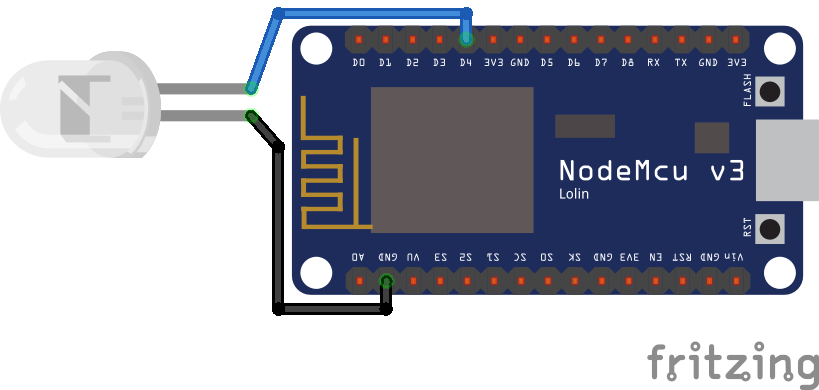
\includegraphics[height=2.5in]{figures/nodemcu-test1.png}
\caption[Montaje placa nodeMCU con led]{Esquema de montaje de led en una placa nodemcu}
    \label{figure1}
\end{figure}

A continuación debe compilarse el proyecto y subirse a la placa, una vez terminado el proceso, el led debe parpadear según lo programado:

\begin{verbatim}
    arduino-cli compile --fqbn esp8266:esp8266:nodemcuv2 test/test
    arduino-cli upload -p /dev/ttyUSB0 --fqbn esp8266:esp8266:nodemcuv2 test/test
\end{verbatim}

Habiendo verificado el proceso de subida es necesario probar que la conexión inalámbrica y la comunicación mediante el protocolo \gls{mqtt} es correcta, con un código distinto. Instanciar un nuevo proyecto, incluir el código, subir el sketch en la placa y probar la comunicación de la placa con el servidor. Es necesario además agregar las librerías necesarias, en el caso que ocupa este proyecto se utiliza la librería PubSubClient de Nick O'Leary, un cliente ligero de MQTT que posee buena estabilidad y facil integración en código.

\begin{verbatim}
    cd ~/Arduino
    arduino-cli lib search PubSubClient
    arduino-cli lib install "PubSubClient"
    arduino-cli sketch new testmqtt
    nano test/testmqtt.ino
\end{verbatim}

El código de prueba de \gls{mqtt} incluye la librería de ESP8266WiFi.h que no es necesario añadir mediante el instalador de librerías, ya que este viene incluido en el core de tarjetas de terceros que se incluyo anteriormente para el chip esp8266. De esta forma, el código incluye los parámetros de conexión \gls{wifi} para el adaptador de red inalámbrico del nodo principal y la conexión al servicio de \gls{mqtt} así como la publicación de topics. El siguiente, es un ejemplo básico para hacer pruebas es una ligera modificación del ejemplo contenido en la ruta \path{~/Arduino/libraries/PubSubClient/examples/mqtt_basic/mqtt_basic.ino}.


\begin{verbatim}
#include <ESP8266WiFi.h>
#include <PubSubClient.h>

const char* ssid = "edomus";
const char* password = "sistemaguardian1970.";
const char* mqtt_server = "192.168.4.1";

WiFiClient espClient;
PubSubClient client(espClient);
char msg[50];
long lastMsg = 0;
int value = 0;

 
void setup_wifi() {
  delay(10);
  // We start by connecting to a WiFi network
  WiFi.begin(ssid, password);
  while (WiFi.status() != WL_CONNECTED) {
    delay(500);
  }
  randomSeed(micros());
}
 
void callback(char* topic, byte* payload, unsigned int length) {
  // Switch on the LED if an 1 was received as first character
  if ((char)payload[0] == '1') {
    digitalWrite(BUILTIN_LED, LOW);   // Turn the LED on (Note that LOW is the voltage level
    // but actually the LED is on; this is because
    // it is acive low on the ESP-01)
  } else {
    digitalWrite(BUILTIN_LED, HIGH);  // Turn the LED off by making the voltage HIGH
  }
}
 
void reconnect() {
  // Loop until we're reconnected
  while (!client.connected()) {
    // Create a random client ID
    String clientId = "nodemcuClient-test";
    clientId += String(random(0xffff), HEX);
    
    // Attempt to connect
    if (client.connect(clientId.c_str())) {
      client.publish("outTopic", "hello world");
      client.subscribe("*/test");
    } else {
      delay(5000);
    }
  }
}

void setup() {
  pinMode(BUILTIN_LED, OUTPUT);     // Initialize the BUILTIN_LED pin as an output
  setup_wifi();
  client.setServer(mqtt_server, 1883);
  client.setCallback(callback);
}
 
void loop() {
  if (!client.connected()) {
    reconnect();
  }
  client.loop();
  long now = millis();
  
  if (now - lastMsg > 2500) {
    lastMsg = now; 
    ++value;
    snprintf (msg, 50, "hello world #%ld", value);
    client.publish("test/msg", msg);
  }
}
\end{verbatim}

Una vez subido el sketch a la placa según los pasos anteriormente indicados, podemos realizar una llamada a la placa mediante el cliente de \gls{mqtt} instalado en el nodo principal. El cual generara una salida de texto sin fin. Con esto, queda probado que el proceso de subida y la placa están en condiciones óptimas de funcionamiento.

\begin{verbatim}
    mosquitto_sub -h localhost -t test/msg
\end{verbatim}

\section{Scritps de generación de sckets placas nodeMCU desde Raspberry Pi}
\label{AppendiA:Key5}

Crear un sketch mediante un script puede variar en su complejidad en el grado de cuantos argumentos reciba y que tan flexible se desea que sea su comportamiento. Sea cual sea el tipo de sketch que se busque crear, se debe mantener una estructura de carga de librerías y constantes, un constructor y un bucle de ejecución. Considerando las necesidades del proyecto, se requiere que el script reciba los siguientes argumentos de entrada:

\begin{itemize}
  \item Modelo de la placa microcontroladora en la que se sube el sketch.

  \item Modelo del sensor/actuador que va a conectarse en el GPIO de la placa microcontroladora.

  \item Valor numérico del pin de conexión de I/O en el que se conectara el sensor/actuador.
  
  \item Nombre de la estancia en la que se planea ubicar la placa microcontroladora.
\end{itemize}

El objetivo ultimo del \gls{script} es generar un \gls{sketch} de Arduino que pueda compilarse correctamente, sin embargo, hasta que se reciben los argumentos solo es posible disponer de una plantilla genérica con secciones que deben ser rellenadas en base a las opciones. El modelo de plantilla básico puede constituirse con código previamente escrito en diferentes ficheros para luego ser ordenadamente ensamblada en un único fichero de código. En el caso de este proyecto se creara una estructura de carpetas constituida por un directorio principal, el script generador, un directorio con las secciones de código común a todos los sketchs y directorios separados para cada sensor/actuador disponible en la aplicación. Para la prueba inicial incluiremos el código del sensor DHT11 para un configurar una placa detectora de temperatura y humedad. En términos generales, un sensor/actuador requiere de 3 bloques de código que integrar en código común, las librerías y constantes, la configuración inicial del setup, y el código del bucle que sera requerido por el protocolo \gls{mqtt} para responder al servidor.

\begin{verbatim}
    cd ~
    mkdir sketchgenerator
    touch sketchgenerator/sketchgenerator
    mkdir sketchgenerator/general
    touch sketchgenerator/general/loop
    touch sketchgenerator/general/setup
    mkdir sketchgenerator/dht
    touch sketchgenerator/dht/dht11Lib
    touch sketchgenerator/dht/dht11Loop
    touch sketchgenerator/dht/dht11Setup
\end{verbatim}

Con esta estructura, el \gls{script} tendra que construir un ficehro de extensión .ino válido en la ruta de destino necesaria para que posteriormente arduino-cli pueda compilarlo y subirlo a la placa microcontroladora conectada a un puerto USB del nodo principal. Primero consideraremos el codigo de uso comun a todos los \gls{sketch}.

\begin{verbatim}
    nano sketchgenerator/general/setup
\end{verbatim}

Considerando que el sensor DHT11 posee cierto código que se incluye en la función setup, se usara una cadena de caracteres a modo de centinela, el cual sera sustituido por el código definido en un fichero concreto (dht11Setup, en este caso) situado en el directorio del sensor definido por los argumentos del srcipt generador. Dicho centinela en este codigo aparece como \verb|SETUP_THING|.

\begin{verbatim}
long lastMsg = 0;
char msg[50];
int value = 0;

void setup() {
  pinMode(BUILTIN_LED, OUTPUT);
  setup_wifi();
  client.setServer(mqtt_server, 1883);
  client.setCallback(callback);

  SETUP_THING
}

void setup_wifi() {
  delay(10);
  WiFi.begin(ssid, password);
  while (WiFi.status() != WL_CONNECTED) {
    delay(500);
  }
}

void callback(char* topic, byte* payload, unsigned int length) {
  if ((char)payload[0] == '1') {
    digitalWrite(BUILTIN_LED, LOW);
  } else {
    digitalWrite(BUILTIN_LED, HIGH);
  }
}

void reconnect() {
  while (!client.connected()) {
    if (client.connect("ESP8266Client")) {
      client.publish("outTopic", "hello world");
      client.subscribe("inTopic");
    } else {
      delay(5000);
    }
  }
}
\end{verbatim}

El siguiente segmento de código común corresponde al bucle sin fin de un \gls{sketch}. Al igual que en el caso anterior, una sección del código deberá ser rellenada por las particularidades del sensor. Para este caso se ha definido un centinela \verb|MAIN_BODY|.

\begin{verbatim}
    nano sketchgenerator/general/loop
\end{verbatim}

\begin{verbatim}
void loop() {
if (!client.connected()) {
    reconnect();
  }
  client.loop();
  long now = millis();
  if (now - lastMsg > 2500) {
    lastMsg = now;
    MAIN_BODY
  }
}
\end{verbatim}

Para las secciones de código de un sensor como el DHT se requiere de las librerías, funciones auxiliares y constantes propias.
\begin{verbatim}
    nano sketchgenerator/dht/dht11Lib
\end{verbatim}

\begin{verbatim}
#include <Adafruit_Sensor.h>
#include <DHT.h>
#include <DHT_U.h>
#define DHTPIN ARGUMENT_PIN
#define DHTTYPE DHT11
DHT dht(DHTPIN, DHTTYPE);
\end{verbatim}

Tambien es necesario el segmento de codigo que se incluye en la fución setup.
\begin{verbatim}
    nano sketchgenerator/dht/dht11Lib
\end{verbatim}

\begin{verbatim}
dht.begin();
\end{verbatim}

Y por ultimo el segmento de código que sera invocado en la función loop que incluye la respuesta del cliente \gls{mqtt}. Este segmento de código también incluye centinelas que deben ser sustituidos en base a los argumentos del generador de \gls{sketch}, ya que de otra forma no seria posible definir los topics a los que responderá la placa cuando el nodo solicite información.
\begin{verbatim}
    nano sketchgenerator/dht/dht11Lib
\end{verbatim}

\begin{verbatim}
float h = dht.readHumidity();
float t = dht.readTemperature();
if (isnan(h) || isnan(t))
{
    snprintf (msg, 75, "{'status':'error', 'message':'Error in DHT11 sensor'}", value);
    client.publish("nodemcudht11", msg);
}
else
{
    snprintf (msg, 75, "'%f'", t);
    client.publish("TOPIC_PLACA/temp", msg);
    snprintf (msg, 75, "'%f'", h);
    client.publish("TOPIC_PLACA/hum", msg);
}
\end{verbatim}

Con todo este código por segmentado puede constituirse un \gls{sketch} valido siempre que se encadene en el orden correcto con las sustituciones adecuadas. El script se ejecutara en el entorno de \verb|Bash|, y realizara la recepción de los argumentos, validación de los mismos y verificación de las rutas de los ficheros de donde se obtendrán los segmentos de codigo de cada parte. Serán unidos y escritos en un fichero situado en la ruta de un proyecto de Arduino que actuara como contenedor para las compilaciones. El srcipt ademas dispone de los credenciales necesarios para la conexión \gls{wifi} al nodo y el servicio de \gls{mqtt}.

\begin{verbatim}
    nano sketchgenerator/sketchgenerator
\end{verbatim}

\begin{verbatim}
#!/bin/bash

destinyPath=../sketchbook/nodemcu.ino

BASICLIBRARIES="#include <ESP8266WiFi.h>\n#include <PubSubClient.h>"

echo -e $BASICLIBRARIES "\n\n"> $destinyPath

#$1 path to sensor
#$2 pint for I/O in sensor
[ $# -eq 0 ] && { echo "Usage: $1 sensor path"; exit 1; }
[ ! -f "$1" ] && { echo "Error: $1 file not found."; exit 2; }
file=$1
pin="D$2"
#Si fichero existe y no es vacio
if [ -s $file ]
then
        while IFS= read -r line
        do
        replace="${line/ARGUMENT_PIN/$pin}"
        echo -e $replace >> $destinyPath
        done < "$file"
else
        echo -e "FICHERO SOLICITADO NO EXISTE\n"
        exit
fi

ACCESS_POINT="const char* ssid = \"edomus\";\n"
PASSWORD="const char* password = \"sistemaguardian1970.\";\n"
MQTT_SERVER="const char* mqtt_server = \"192.168.4.1\";\n"
WIFI_CONST="WiFiClient espClient;\n"
WIFI_CLI="PubSubClient client(espClient);\n"


echo -e $ACCESS_POINT$PASSWORD$MQTT_SERVER$WIFI_CONST$WIFI_CLI >> $destinyPath



#GET SETUP FOR SELECTED THING
thingSetup=""
[ ! -f "$1Setup" ] && { echo "Error: $1Setup file not found."; exit 2; }
if [ -s "$1Setup" ]
then
        while IFS= read -r line
        do
        thingSetup+=$line
        done < "$1Setup"
fi

[ ! -f "general/setup" ] && { echo "Error: setup file not found."; exit 2; }
if [ -s "general/setup" ]
then
        while IFS= read -r line
        do
        main="${line/SETUP_THING/$thingSetup}"
        echo -e $main >> $destinyPath
        done < "general/setup"
fi
\end{verbatim}
% +--------------------------------------------------------------------+
% | Appendix B Page (Optional)                                         |
% +--------------------------------------------------------------------+

\cleardoublepage

\chapter{Troubleshooting}
\label{AppendiB:Key1}

\section{Proceso de subida de sckets pacas nodeMCU desde Raspberry Pi}
\label{AppendiB:Key2}

sudo apt-get install git raspberrypi-kernel-headers build-essential dkms
https://github.com/juliagoda/CH341SER
nano328


\section{Error en la instlación de mosquitto}
\label{AppendiB:Key3}
-- Error

The following packages have unmet dependencies:
 mosquitto : Depends: libssl1.0.0 (>= 1.0.0) but it is not installable
             Depends: libwebsockets3 (>= 1.2) but it is not installable

--- solucion
https://theembeddedlab.com/tutorials/install-mosquitto-on-a-raspberry-pi/

% +--------------------------------------------------------------------+
% | Enter text for your Appendix page in the space below this box.     |
% |                                                                    |
% +--------------------------------------------------------------------+

\section{Margenes de error del sensor DHT11}
\label{AppendiB:key4}
sensor DHT version 1.4. Se debe realizar una prueba de contacto con un script que nos muestre la información por pantalla para verificar que las conexiones del sensor a la rapsberry son correctos. Este primer script es un bucle infinito de mediciones de temperatura y humedad cada poco segundos. Hay una justificación para elegir un bucle sobre una única medida del sensor y está fundamentada en el margen de error inicial de las medidas. Si bien el sensor DTH11 es una opción muy común por su bajo coste y facilidad de implementación (este sensor se caracteriza por tener la señal digital calibrada por lo que asegura una alta calidad y una fiabilidad a lo largo del tiempo, ya que contiene un microcontrolador de 8 bits integrado. Está constituido por dos sensores resistivos (NTC y humedad) - revisar esta info y contrastarla contra ésta: \url{https://programarfacil.com/blog/arduino-blog/sensor-dht11-temperatura-humedad-arduino/} ), ademas de manejar señales digitales que no se ven afectadas por las fluctuaciones de voltaje, tiene algunas contrapartidas que deben tenerse en cuenta. Se necesita un tiempo mínimo de espera entre medidas (de al menos 1 segundo), hecho que no agrava particularmente su desempeño en entornos cerrados como una casa, ya que las variaciones de temperatura y humedad no son bruscas, aun así existen estrategias para reducir estos tiempos, por ejemplo, usar la función millis() de Arduino, el cual nos da el tiempo en milisegundos desde que empieza a ejecutarse el código, De esta forma evitamos la pausa de los 2 segundos, pero no el tiempo que demora en hacer la lectura, que es de aproximadamente  250 milisegundos, el cual lo pueden notar si realizan el ejemplo anterior, en donde se hace parpadear el led interno de la placa (Pin 13) con pausas de 100ms (tomado de \url{https://naylampmechatronics.com/blog/40_Tutorial-sensor-de-temperatura-y-humedad-DHT1.html}). Otro problema que abordar es que las primeras lecturas tienen un margen de error de unos +-2 grados Celsius y +-5\% de humedad relativa en las primeras 4 lecturas. Esto generará un problema a la hora de tomar lecturas instantáneas si el sensor no se encuentra ya operando cuando se solicita el dato.

\end{document}
